% !TEX program = xelatex
% =====================================================================
%  SLIM-FRNet —— 大学生创新创业训练计划结项研究报告
%  编译： xelatex main → bibtex main → xelatex main ×2
%  或：   latexmk -xelatex main.tex
% =====================================================================
\documentclass[UTF8, fontset=windows, a4paper, 11pt]{ctexart}

% ---------- 版面 ----------
\usepackage[top=2.4cm, bottom=2.4cm, left=2.6cm, right=2.6cm]{geometry}
\usepackage{setspace}
\usepackage{silence}
\WarningFilter{latexfont}{Font shape}
\WarningFilter{latexfont}{Some font shapes}
\setstretch{1.28}
\setlength{\parskip}{2pt}

% ---------- 数学与符号 ----------
\usepackage{amsmath, amssymb, bm}

% ---------- 图表 ----------
\usepackage{graphicx}
\usepackage{booktabs, tabularx, multirow, threeparttable}
\usepackage{float}
\usepackage[font=small, labelfont=bf]{caption}
\usepackage{subcaption}
\usepackage{xcolor}
\usepackage{tikz}
\usetikzlibrary{positioning, arrows.meta, shapes.geometric, fit, backgrounds, calc}

% ---------- 列表与代码 ----------
\usepackage{enumitem}
\setlist[itemize]{leftmargin=2em, itemsep=1pt, topsep=2pt}
\setlist[enumerate]{leftmargin=2em, itemsep=1pt, topsep=2pt}
\usepackage{listings}
\lstset{
    basicstyle=\ttfamily\footnotesize,
    keywordstyle=\color[rgb]{0.13,0.29,0.53}\bfseries,
    commentstyle=\color[rgb]{0.35,0.45,0.35}\itshape,
    stringstyle=\color[rgb]{0.55,0.25,0.15},
    numbers=left, numberstyle=\tiny\color{gray}, numbersep=6pt,
    frame=single, rulecolor=\color{gray!40},
    breaklines=true, showstringspaces=false,
    columns=fullflexible, keepspaces=true,
    extendedchars=false, escapeinside={(*@}{@*)},
}

% ---------- 页眉页脚 ----------
\usepackage{fancyhdr}
\pagestyle{fancy}
\fancyhf{}
\fancyhead[L]{\small SLIM-FRNet：轻量级可复现合成指纹数据集生成平台}
\fancyhead[R]{\small\leftmark}
\fancyfoot[C]{\small\thepage}
\renewcommand{\headrulewidth}{0.4pt}

% ---------- 标题样式 ----------
\usepackage{titlesec}
\usepackage{tocloft}
\setlength{\cftbeforetoctitleskip}{0pt}
\setlength{\cftaftertoctitleskip}{4pt}
\setlength{\cftbeforesecskip}{1.0pt}
\setlength{\cftbeforesubsecskip}{0.2pt}
\renewcommand{\cftsecleader}{\cftdotfill{\cftdotsep}}
\titleformat{\section}{\large\bfseries}{\thesection}{0.6em}{}
\titlespacing*{\section}{0pt}{1.2ex plus .3ex}{0.8ex}
\titleformat{\subsection}{\normalsize\bfseries}{\thesubsection}{0.5em}{}
\titlespacing*{\subsection}{0pt}{1.0ex plus .2ex}{0.6ex}

% ---------- 链接 ----------
\usepackage[colorlinks=true, linkcolor=black, citecolor=black, urlcolor=blue!55!black,
            bookmarksnumbered=true]{hyperref}

% ---------- 参考文献（GB/T 7714） ----------
\usepackage[numbers, sort&compress]{natbib}
\bibliographystyle{gbt7714-numerical}

% ---------- 自定义命令 ----------
\newcommand{\name}{SLIM-FRNet}
\newcommand{\px}{\,\mathrm{px}}
% ctex 的 fontset=windows 没有仿宋斜体，缺字时静默替换；补一个伪斜体兜底
\IfFontExistsTF{FangSong}{\setCJKfamilyfont{zhfs}[AutoFakeSlant=0.18]{FangSong}}{}
\newcommand{\unit}[1]{\,\mathrm{#1}}
\newcommand{\figref}[1]{图~\ref{#1}}
\newcommand{\tabref}[1]{表~\ref{#1}}

% =====================================================================
\begin{document}

% ---------- 标题 ----------
\begin{center}
    {\LARGE\bfseries \name{}：轻量级可复现合成指纹数据集\\[2pt]
     生成平台的设计、实现与评测\par}
    \vspace{6pt}
    {\large 大学生创新创业训练计划\quad 结项研究报告\par}
\end{center}

\vspace{2pt}
\begin{center}
\begin{tabular}{rl}
    项目名称： & 基于生成模型的合成指纹数据集构建平台 \\
    成果形式： & 桌面应用软件（含命令行接口）、开源代码仓库、实验数据集 \\
    报告日期： & 2026 年 10 月 \\
\end{tabular}
\end{center}

\vspace{4pt}
\begin{center}\rule{0.9\textwidth}{0.4pt}\end{center}

% ---------- 摘要 ----------
\section*{摘\quad 要}
\addcontentsline{toc}{section}{摘要}

生物特征识别模型的训练与评测高度依赖数据，而真实指纹数据受隐私法规与采集成本
限制，难以大规模获取与分发。合成指纹生成因此成为一条现实可行的替代路径。
本文介绍自主设计与实现的桌面平台 \name{}：它以复刻 SFinGe 方法学为核心，
把``手指轮廓—奇异点—方向场—频率图—Gabor 脊线—捺印—数据增强''整条链路封装为
图形界面下的一键操作，并在此基础上解决三个工程问题——\textbf{轻量}（仅 4 个核心
第三方依赖）、\textbf{可复现}（种子树 + 配置指纹 + 环境快照 + 全量校验和的四要素
闭环）、\textbf{可扩展}（六个插件维度均以注册表解耦）。

我们在 AMD Ryzen 9 8945HX（32 线程）、Windows 11、Python 3.13 环境下完成了
72 样本的正式实验：单张主指纹渲染中位耗时 $0.57\unit{s}$，端到端单线程吞吐
$3.42$ 样本/秒、8 线程 $6.33$ 样本/秒；质量分（NFIQ 2 风格，$0$--$100$）均值
$68.7$、中位 $71.6$；细节点均值 $80.6$；脊线周期中位 $11.0\px$、占空比 $0.50$，
与真实 500\,dpi 指纹（$8$--$12\px$）处于同一量级；同配置同种子两次独立运行，
504 个产出文件的 SHA-256 校验和逐字节一致。

实验过程中我们还定位并修复了一个会静默产出空白样本的缺陷（光度类增强算子被
错误地作用在二值掩模上，导致掩模整块被清空），修复后空白样本比例由 $5.6\%$
降至 $0$。本文最后讨论了该平台与 SFinGe 的差异、当前的局限（缺少识别级评测、
脊线周期略偏粗、并行加速比有限）以及后续工作。

\vspace{4pt}
\noindent\textbf{关键词：}\ 合成指纹；SFinGe；数据增强；可复现性；Gabor 滤波；图形界面

\vspace{2pt}
\begin{center}\rule{0.9\textwidth}{0.4pt}\end{center}

\clearpage
\tableofcontents
\newpage

% =====================================================================
\section{引言}

\subsection{研究背景与意义}

指纹识别是应用最成熟的生物特征识别技术之一\cite{maltoni2009}。近年基于深度
学习的指纹算法（细节点检测、质量评估、特征嵌入）对数据规模与多样性的要求
迅速提高，而真实指纹数据的获取面临三重约束：其一，指纹属于敏感个人生物特征，
受《个人信息保护法》《通用数据保护条例》等法规严格限制，跨机构共享几乎不可行；
其二，大规模采集需要专用活体传感器与受试者配合，成本高、周期长；其三，公开
数据集（如 FVC 系列\cite{maio2002}、NIST SD4\cite{watson1992}）规模有限且
身份固定，容易导致模型过拟合于特定采集条件。

合成指纹生成提供了另一条路径：由算法直接产生具有真实指纹形态学特征的图像，
并可精确控制类别、质量、形变与增强参数。由于不含任何真实个体信息，合成数据
在隐私与合规上天然安全，也便于按需构造类别均衡、难度可控的训练集与测试集。
SFinGe\cite{cappelli2000,cappelli2004}是这一方向最具影响力的工作，但其原始
实现年代较早、依赖较重、且缺少面向现代研究流程的可复现与批量生产能力。

\subsection{国内外研究现状}

合成指纹的主流方法可归为三类。\textbf{基于模型的方法}从指纹的生成机理出发：
先由少数参数描述手指轮廓与奇异点（core/delta）分布，再依据 Sherlock--Monro
模型\cite{sherlock1994}或零极点模型\cite{vizcaya1996}生成方向场，随后在方向场
约束下用 Gabor 滤波器迭代合成脊线\cite{hong1998}，最后叠加采集过程的退化。
SFinGe 是这一路线的代表，其生成结果已被用于多项识别算法的训练与评测。

\textbf{基于深度学习的方法}则以数据驱动方式学习真实指纹的分布。例如 Cao 与
Jain 提出的由细节点重建指纹图像的方案\cite{cao2015}，以及随后出现的各类
生成对抗网络方法。这类方法在视觉逼真度上表现突出，但需要大量真实数据作为
训练前提，且生成过程的可控性与可复现性较弱——这与``用合成数据替代真实数据''
的初衷存在一定张力。

\textbf{面向工程可用性的工作}关注的是另一组问题：批量生成、参数化控制、质量
筛选与数据集的标准化组织。真实研究流程中，研究者往往需要在几十分钟内产出一个
类别均衡、划分无泄漏、元数据完备的数据集，并能在论文中精确复现它；这类需求
恰恰是多数研究原型所欠缺的。

\subsection{本文工作与贡献}

本文的工作是把上述第三条路线做扎实：在复刻 SFinGe 生成链的基础上，重建一套
面向``可用、可查、可复现''的桌面平台。主要贡献如下：

\begin{enumerate}
    \item \textbf{完整的生成链与工程化平台。}实现从手指轮廓、奇异点、方向场、
          频率图到 Gabor 迭代脊线，再到捺印建模、数据增强、质量评估、细节点
          标注、数据集导出的全链路，并提供 8 页图形界面与命令行双入口。
    \item \textbf{可复现性的机制化保证。}设计与实现基于 SHA-256 的五级种子树
          （数据集→身份→手指→捺印→增强），配合配置指纹、环境快照
          与全量校验和，使``同配置同种子逐字节可复现''成为可自动验证的性质，
          而非口头承诺。
    \item \textbf{轻量依赖与可扩展架构。}核心仅依赖 numpy、OpenCV、pydantic、
          PyYAML 四个库；GUI 通过兼容层同时支持 PySide6 与 PyQt6。六个插件
          维度（生成后端、捺印变形、传感器、TTA 算子、质量评估、细节点）均以
          注册表解耦，新增算子无需改动 GUI 与管道。
    \item \textbf{面向真实感的质量标定与缺陷修复。}以真实 500\,dpi 指纹的脊线
          周期为基准标定生成参数，并用回归测试固定该性质；在实验中定位并修复了
          一个导致 $5.6\%$ 样本静默变为空白的掩模缺陷。
\end{enumerate}

% =====================================================================
\section{相关工作}

\subsection{基于模型的合成指纹生成}

SFinGe 的核心思想是``用尽可能少的参数生成尽可能真实的指纹''\cite{cappelli2000}。
其流程可概括为：先生成手指轮廓与奇异点，再由奇异点位置确定方向场的零极点分布，
用方向场引导 Gabor 滤波器迭代地``生长''脊线，最后模拟按压形变与传感器噪声。
其中方向场建模经历了从 Sherlock--Monro 的复数多项式模型\cite{sherlock1994}
到 Vizcaya--Gerhardt 的非线性模型\cite{vizcaya1996}的演进；脊线增强则普遍采用
Gabor 滤波\cite{hong1998}，因为它能在保持脊线方向选择性的同时抑制噪声。

本文的实现沿用了这一方法学，但在三处做了工程化改造：频率图改用多倍频 Perlin
噪声\cite{perlin1985}在奇异点附近调制；迭代在缩小网格上进行以降低卷积代价，
并按缩放比例正确换算频率；捺印阶段把``按压形变—传感器特性—随机退化''拆成
可独立开关的三段。

\subsection{质量评估与细节点}

指纹图像质量评估的工业标准是 NFIQ 系列\cite{tabassi2004,tabassi2021}，其第二版
以随机森林融合多类特征，输出 $0$--$100$ 的分数与 1--5 的质量等级（1 为最好）。
商用实现不开源，且与特定厂商的传感器特性耦合。本文实现了一个\textbf{NFIQ 2 风格}
的自研评分器：以脊线清晰度、对比度、方向一致性、有效面积、脊线周期合理性五项
加权，输出同向的分数与等级——好处是零外部依赖、跨平台一致且完全确定，代价是
未经 NIST 标定，不能与官方分数直接比较。

细节点提取沿用经典的``细化 + 交叉数''路线：先用 Zhang--Suen 并行细化\cite{zhang1984}
得到单像素骨架，再以 $3\times3$ 邻域的交叉数判别末梢与分叉，配合边界裁剪与最小
间距抑制伪点；可选导出 ISO/IEC 19794-2 风格的模板\cite{iso19794}。

\subsection{可复现性}

可复现性已成为计算科学研究的基本要求\cite{sandve2013}。对合成数据而言，它比
通常意义上的``代码可运行''更强：同一份配置与种子必须产生\textbf{逐字节相同}的
数据，否则后续在论文中报告的识别精度将无法被他人复核。本文因此把可复现性设计
成机制：种子由 SHA-256 派生而非 Python 的 \texttt{hash()}（后者受哈希随机化
影响，跨进程不稳定），数据集名称参与种子派生，配置文件、环境快照与校验和随
数据集一同落盘。

% =====================================================================
\section{系统设计}

\subsection{总体架构}

系统采用严格单向的分层结构（\figref{fig:arch}）：\texttt{gui} $\to$ \texttt{app}
$\to$ \{\texttt{pipeline}, \texttt{core}\} $\to$ \texttt{plugins} $\to$
\texttt{legacy}。核心约束是\textbf{下层不得依赖上层，且除 GUI 外任何模块不得
导入 Qt}——这使得生成链可以在无图形环境的服务器或 CI 中完整运行，也是自动化
测试能在无显示器条件下跑通 916 个用例的前提。

\begin{figure}[H]
\centering
\begin{tikzpicture}[
    node distance=4mm,
    box/.style={draw=black!55, rounded corners=3pt, fill=#1, minimum height=8.5mm,
                text width=0.86\textwidth, align=left, inner sep=4pt, font=\small},
    box/.default={white},
    lbl/.style={font=\scriptsize\bfseries, text=black!70, anchor=south west},
    arr/.style={-{Latex[length=2mm]}, draw=black!60, line width=0.5pt},
]
\node[box=blue!7] (gui) {\textbf{gui} —— 8 页图形界面、主题、控件库、Qt 双绑定兼容层；
    只通过应用服务层读写配置};
\node[box=green!7, below=of gui] (app) {\textbf{app} —— 应用服务层：生成服务、预览服务、
    导出、统计；负责线程编排与回调};
\node[box=orange!8, below=of app] (core) {\textbf{pipeline} + \textbf{core} —— 算子链选择、
    样本管道、调度器、计划器、种子树、Manifest、存储布局};
\node[box=red!6, below=of core] (plug) {\textbf{plugins} —— 六个可替换维度：生成后端、
    捺印变形、传感器、TTA 算子、质量评估、细节点};
\node[box=black!5, below=of plug] (leg) {\textbf{legacy} —— 已验证的渲染内核（轮廓、奇异点、
    方向场、频率图、Gabor）与 19 个退化算子};
\draw[arr] (gui) -- (app);
\draw[arr] (app) -- (core);
\draw[arr] (core) -- (plug);
\draw[arr] (plug) -- (leg);
\node[lbl] at ([xshift=2mm,yshift=1mm]gui.north west) {依赖方向（上层 $\to$ 下层，不可逆）};
\node[draw=black!30, dashed, rounded corners=2pt, fit=(gui)(leg), inner sep=3pt] {};
\end{tikzpicture}
\caption{系统分层架构。箭头表示依赖方向；\texttt{core}、\texttt{pipeline}、
\texttt{app}、\texttt{plugins}、\texttt{legacy}、\texttt{config} 均不导入 Qt。}
\label{fig:arch}
\end{figure}

\subsection{生成链}

一个样本的诞生要经过九个阶段（\figref{fig:chain}）。其中``主指纹''是任务粒度：
同一手指只渲染一次，随后派生出多个捺印与多个增强版本。这一选择使
``每个手指只算一次''成为\textbf{结构性保证}而非缓存优化——增加捺印数量或增强
强度的边际成本因此很低。

\begin{figure}[H]
\centering
\begin{tikzpicture}[
    node distance=3.2mm,
    st/.style={draw=black!55, rounded corners=2pt, fill=#1, minimum height=7mm,
               minimum width=17mm, align=center, font=\scriptsize, inner sep=2pt},
    st/.default={white},
    arr/.style={-{Latex[length=1.8mm]}, draw=black!60},
]
\node[st=blue!8]  (a) {手指轮廓\\5 参数};
\node[st=blue!8, right=of a]  (b) {奇异点\\core/delta};
\node[st=blue!8, right=of b]  (c) {零极点\\方向场};
\node[st=blue!8, right=of c]  (d) {Perlin\\频率图};
\node[st=blue!8, right=of d]  (e) {Gabor\\迭代脊线};
\node[st=orange!12, below=of e] (f) {捺印\\形变/传感器/退化};
\node[st=orange!12, left=of f]  (g) {TTA\\21 算子};
\node[st=green!10, left=of g]   (h) {质量\\五指标};
\node[st=green!10, left=of h]   (i) {细节点\\细化+CN};
\node[st=green!10, left=of i]   (j) {存储\\校验和};
\foreach \s/\t in {a/b,b/c,c/d,d/e} \draw[arr] (\s) -- (\t);
\draw[arr] (e) -- (f);
\foreach \s/\t in {f/g,g/h,h/i,i/j} \draw[arr] (\s) -- (\t);
\node[draw=black!30, dashed, rounded corners=2pt, fit=(a)(e), inner sep=2pt,
      label={[font=\scriptsize\bfseries, text=blue!60!black]above:主指纹（每个手指一次）}] {};
\node[draw=black!30, dashed, rounded corners=2pt, fit=(f)(g), inner sep=2pt,
      label={[font=\scriptsize\bfseries, text=orange!70!black]below:捺印（每指多次）}] {};
\end{tikzpicture}
\caption{单样本生成链。上半部分对每个手指只执行一次，下半部分对每个捺印/增强
各执行一次。}
\label{fig:chain}
\end{figure}

\subsection{可复现性：四要素闭环}

平台把可复现性拆成四个可核对的要素，并随数据集一同落盘：

\begin{enumerate}
    \item \textbf{配置}：\texttt{config.resolved.yaml}，即实际生效的全部参数
          （含默认值展开与命令行覆盖）；
    \item \textbf{种子}：\texttt{runtime.seed}，配合层级种子树可精确重建每一个
          随机决策；
    \item \textbf{版本}：\texttt{environment.json}，记录 Python、numpy、OpenCV、
          pydantic 版本与配置指纹；
    \item \textbf{校验和}：\texttt{checksums/sha256sums.txt}，覆盖数据集内全部文件。
\end{enumerate}

种子树的派生规则如下（\texttt{core/seeds.py}）：以 SHA-256 对
\texttt{"|".join(parts)} 取前 8 字节作为整数，逐层派生出
$\text{dataset} \to \text{identity} \to \text{finger} \to \text{impression} \to \text{tta}$
五级种子。相比 Python 内置 \texttt{hash()}，SHA-256 派生不受 \texttt{PYTHONHASHSEED}
随机化影响，因而跨进程、跨平台稳定。\textbf{数据集名称参与 dataset 级派生}，
这意味着``改名重跑''等价于换了一份数据——这一点在实验设计时极易被误判为
``可复现性失效''（见 \S\ref{sec:repro}）。

\subsection{图形界面}

界面分为三区：左侧 8 页导航、中央配置页、底部状态栏（\figref{fig:gui}）。
页面采用声明式``配置 $\leftrightarrow$ 控件''双向绑定：控件注册一个点号路径，
刷新时自动回填、改动时自动写回，因此新增配置项只需一行注册代码。界面支持
深浅两套主题，并在缺少 PySide6 时自动回退到 PyQt6。

\begin{figure}[H]
\centering
\begin{subfigure}[b]{0.49\textwidth}
    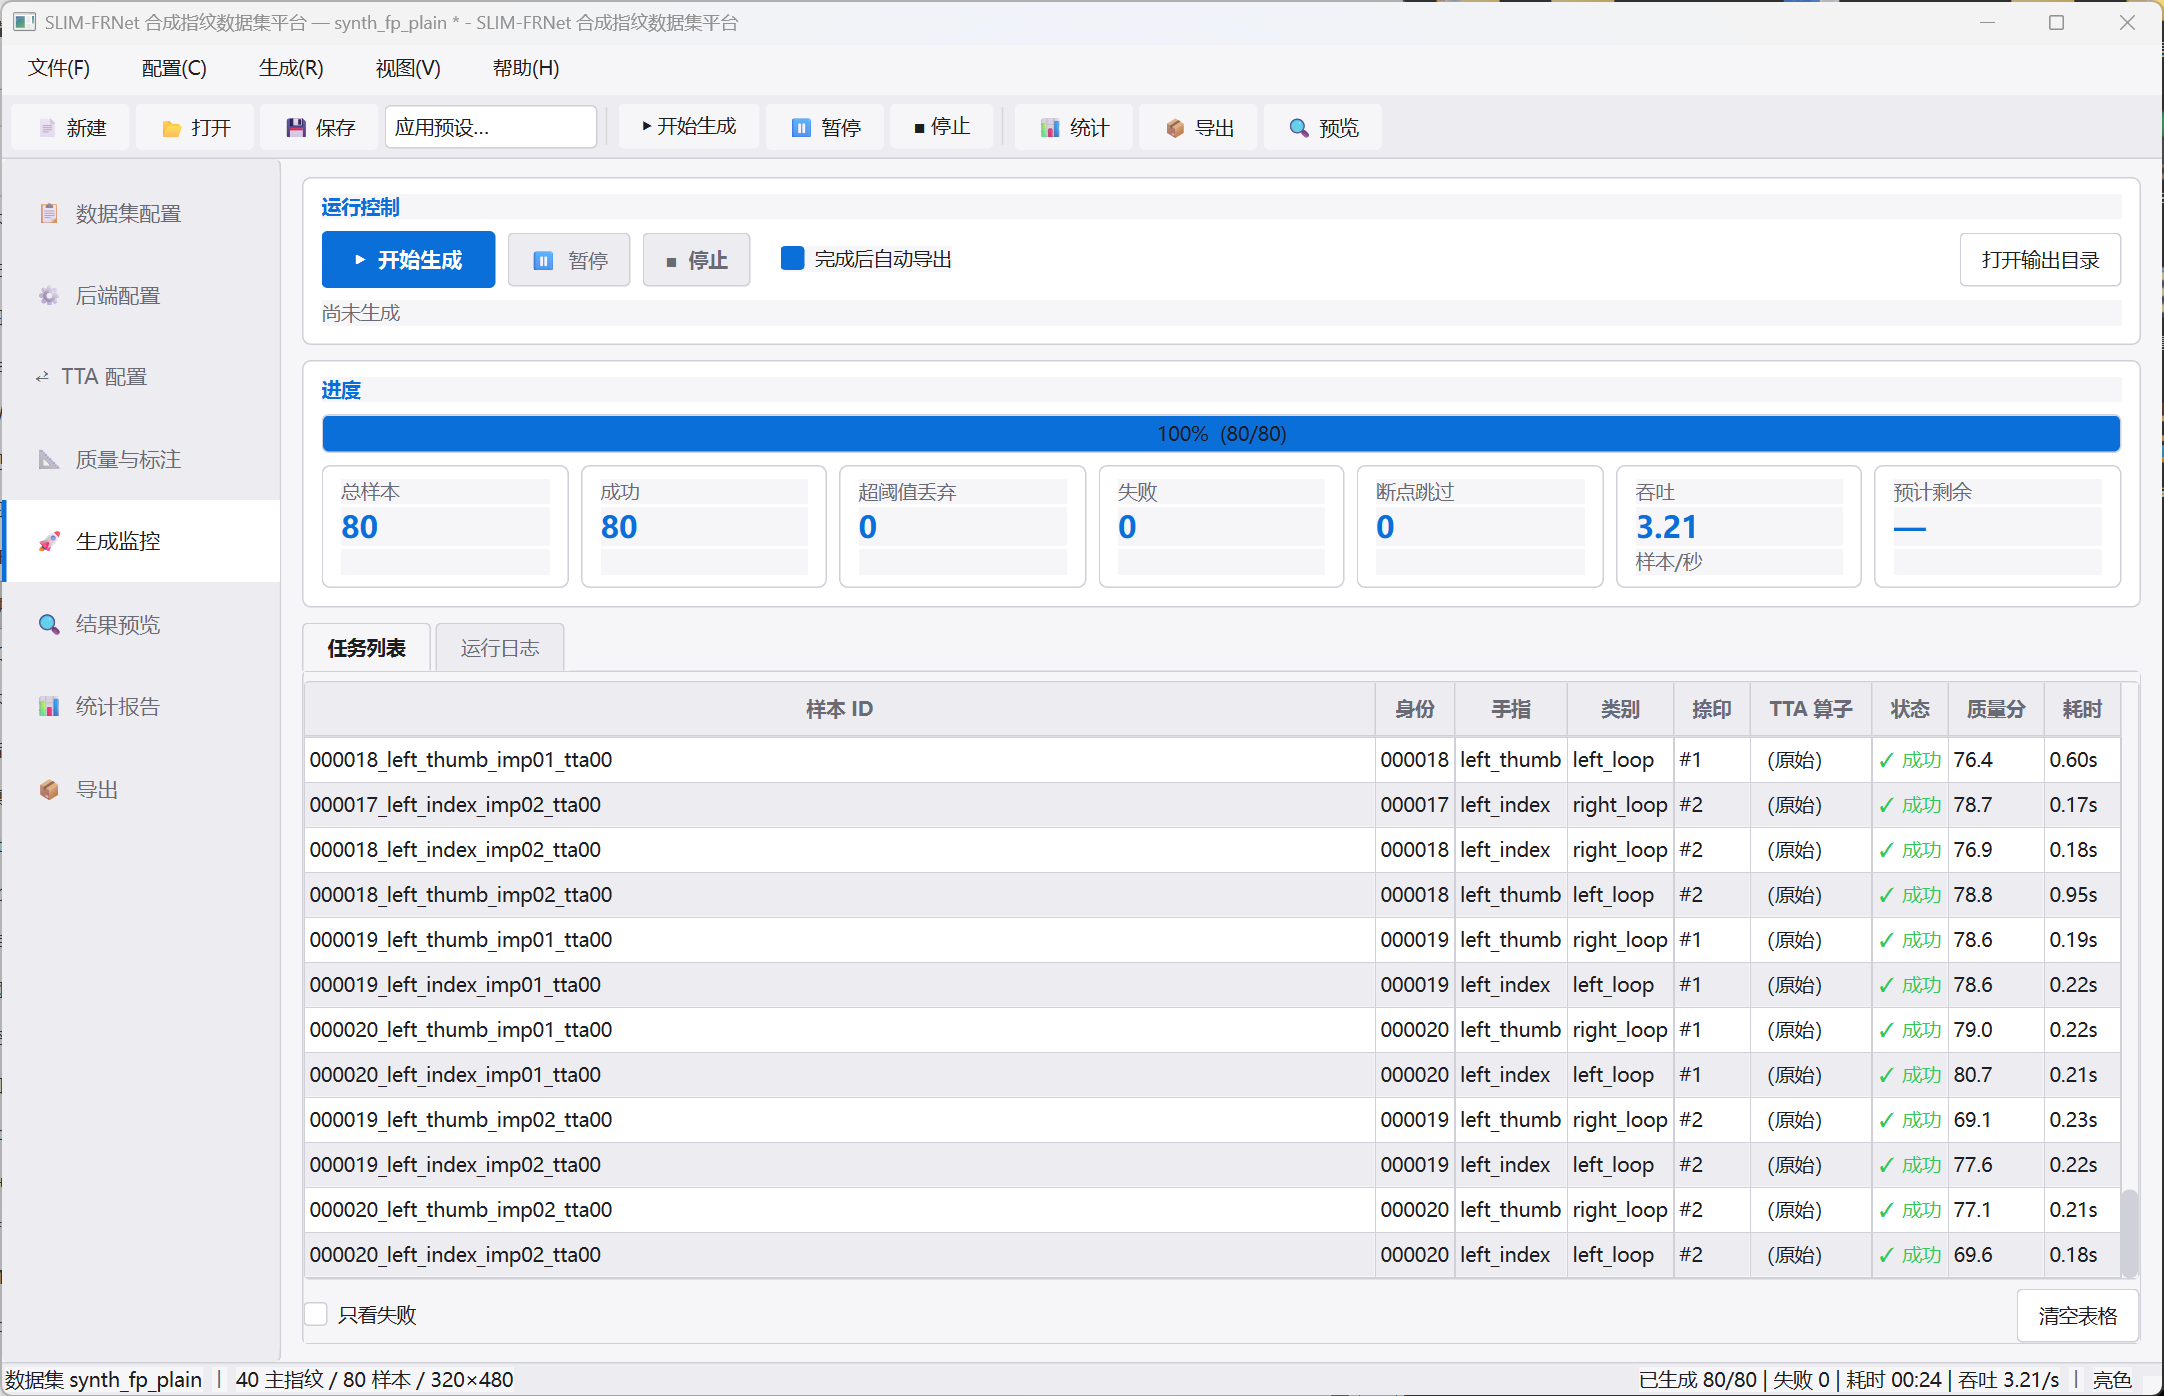
\includegraphics[width=\linewidth]{../docs/screenshots/gui-01-monitor.png}
    \caption{生成监控：进度、实时统计、任务表}
\end{subfigure}\hfill
\begin{subfigure}[b]{0.49\textwidth}
    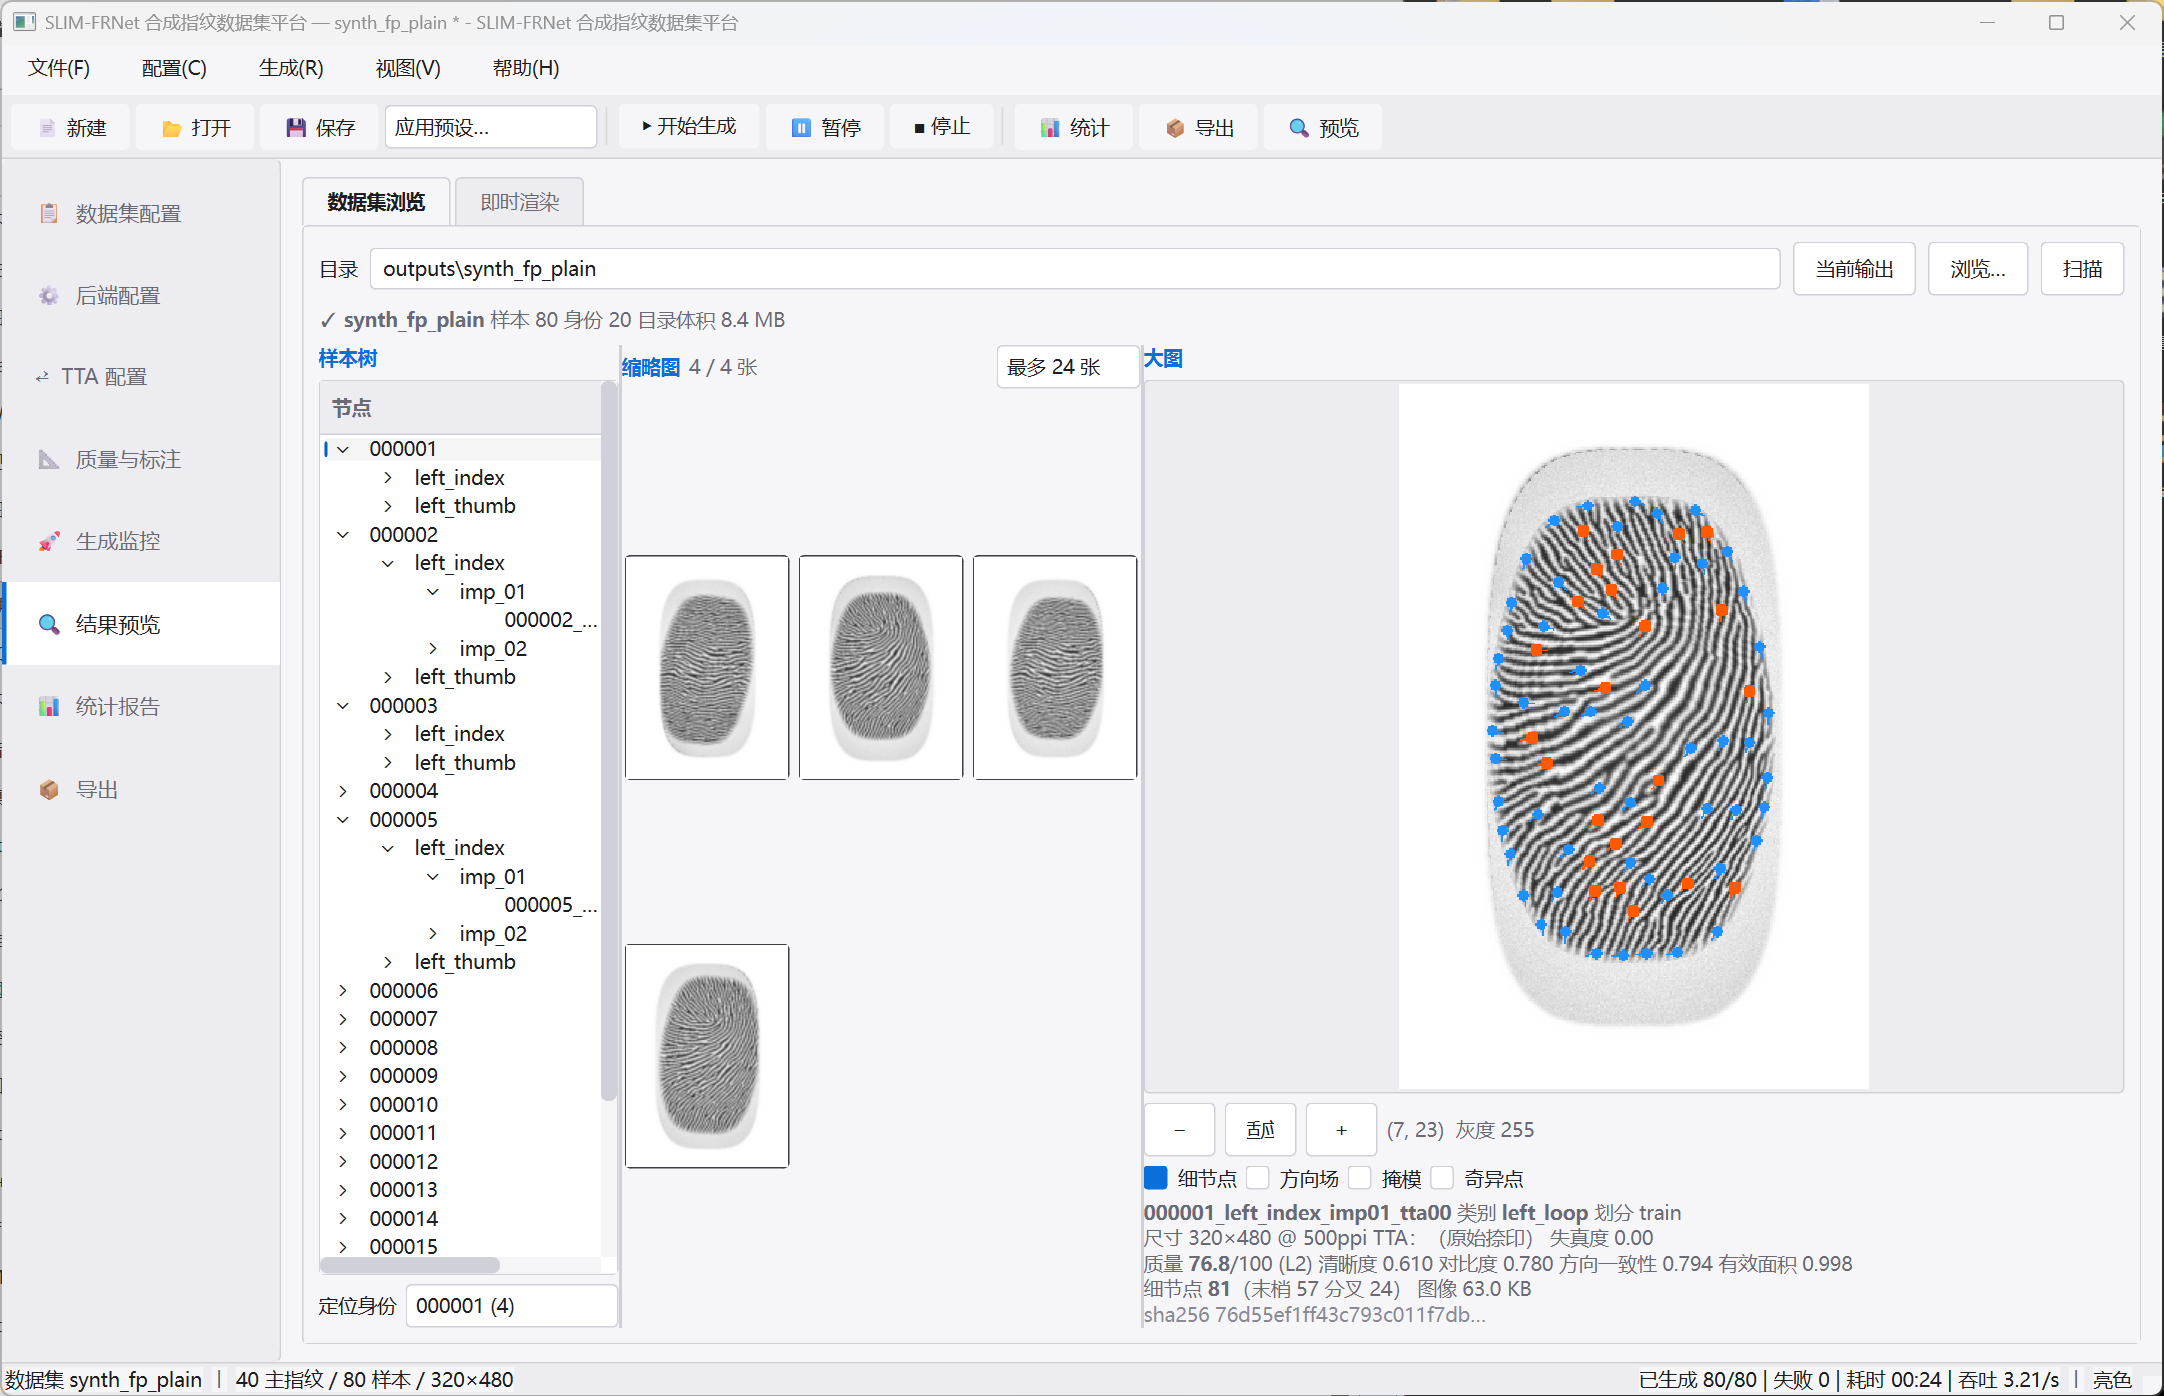
\includegraphics[width=\linewidth]{../docs/screenshots/gui-02-preview.png}
    \caption{结果预览：样本树、缩略图、细节点叠加}
\end{subfigure}
\caption{图形界面示例（浅色主题）。}
\label{fig:gui}
\end{figure}

% =====================================================================
\section{关键实现}

\subsection{方向场：零极点模型}

方向场可由梯度张量法、复数滤波器等多种方法估计\cite{bazen2002,ratha1995}。
本文采用可解析重建的\textbf{零极点模型}：方向场由若干``核心（core，正极点）''与
``三角（delta，负极点）''的位置决定。
记第 $k$ 个奇异点的位置为 $z_k$、电荷为 $q_k \in \{+1,-1\}$，则在像素点 $z$ 处的
复方向角可取为
\begin{equation}
\theta(z) = \frac{1}{2}\sum_{k} q_k \arg(z - z_k) + \theta_0 ,
\label{eq:orientation}
\end{equation}
其中常数项 $\theta_0$ 由全局方向趋势给出。系数 $1/2$ 来自指纹方向场的
\textbf{半周期对称性}：方向场以 $\pi$ 为周期，一条脊线绕奇异点一周方向只转半圈。
式~\eqref{eq:orientation} 在实现上转化为对复数域核函数取角，再做 $[0,\pi)$ 的
归一化，避免了逐点解微分方程的代价。

\subsection{频率图：多倍频 Perlin 调制}

脊线间距在指腹上并非常数，而是在奇异点附近略密、在边缘略疏。本文以
$1/f$ 给出基准周期 $f_0$，再叠加三层 Perlin 噪声\cite{perlin1985}采样值
$n_i \in [-1,1]$：
\begin{equation}
f(x,y) = f_0 \left[1 + \beta \sum_{i=1}^{3} 2^{-i}\, n_i(x,y)\right],
\label{eq:freq}
\end{equation}
其中 $\beta$ 为频率波动比例（默认 $0.25$）。Gabor 核库按``方向 $\times$ 频率''
离散成若干档：每个像素依据其方向与频率索引到对应核，迭代时只需做一次
\texttt{filter2D} 即可。

\subsection{Gabor 迭代与频率换算}

设方向场为 $\theta(x,y)$、频率图为 $f(x,y)$，Gabor 核取
\begin{equation}
g(u,v) = \exp\!\left(-\frac{u^2+v^2}{2\sigma^2}\right)
         \cos\!\left(2\pi f\, u\right),\qquad
(u,v) = \bigl(x\cos\theta + y\sin\theta,\; -x\sin\theta + y\cos\theta\bigr),
\end{equation}
其中 $\sigma$ 由 $f$ 决定，使核在频率 $f$ 处取得最大响应。迭代规则为
``响应为正处保留脊线''：$P_{t+1} = \mathbb{1}\left[\,(g * P_t) > 0\,\right]$，
直至前景像素数变化小于收敛阈值。

为降低卷积代价，迭代在缩放系数 $s$（默认 $0.7$）的网格上进行，收敛后再放大回
原尺寸。\textbf{此处有一个易错点}：频率是``每像素''量，缩放到 $c_w = s\,w$ 的
网格后，同一根手指占据的像素数变为 $s$ 倍，脊线周期变为 $sS$，因此频率必须
变换为
\begin{equation}
f_{\text{coarse}} = \frac{f}{s} = f \cdot \frac{w}{c_w} .
\label{eq:scale}
\end{equation}
早期实现误写为 $f\cdot\frac{c_w}{w}$（乘反），导致脊线周期被系统性放大
$1/s^2 \approx 2$ 倍：实测周期由应有的约 $10\px$ 变为约 $22\px$，
肉眼可见``指纹过稀''。该缺陷不会触发任何功能异常，最终依靠
\S\ref{sec:ridge} 的物理量回归测试才被固定住。

\subsection{捺印建模}

一次捺印由三段可独立开关的处理构成：

\begin{itemize}
    \item \textbf{按压形变}：以位移场 $\bm{d}=(d_x,d_y)$ 描述皮肤受压后的非刚性
          位移，叠加旋转、平移与弹性扰动；位移后未被覆盖的区域还原为采集背景，
          而非变形前的图像（否则会在指边留下弧形残影）。
    \item \textbf{传感器特性}：实现光学、电容、热感三类传感器与一个直通模式。
          光学传感器以对比度压缩、径向暗角与乘性散斑建模；电容传感器额外引入
          椒盐噪声与逐行读出偏置。
    \item \textbf{随机退化}：从 19 个退化算子（模糊、断线、污渍、干湿、遮挡等）
          中随机选取 $1$--$2$ 个施加，模拟真实采集中的非理想因素。
\end{itemize}

\subsection{TTA 算子体系与掩模同源变换}

数据增强共 21 个算子，分六类：几何 6（旋转、平移、缩放、错切、弹性、透视）、
光度 5（亮度、对比度、Gamma、高斯/运动模糊）、噪声 3（高斯、泊松、椒盐）、
压缩 1（JPEG）、遮挡 3（矩形、椭圆、划痕）、传感器 3（光学、电容、热感）。
算子链在样本种子上采样，因此同一样本在任何机器上都得到同一条链；
\texttt{tta\_index = 0} 的样本始终保留未变换的捺印，作为干净对照。

掩模必须与图像\textbf{同源}变换，否则细节点会在背景里产生大量伪点。实现上，
掩模只经过\textbf{改变空间位置或可见性}的算子（几何与遮挡），而光度、噪声、
压缩、传感器四类\textbf{像素值}算子被显式跳过。这一区分是实验阶段修复的缺陷
（见 \S\ref{sec:defect}）：若把亮度算子作用在二值掩模上，偏移量会把前景从
$1.0$ 压到阈值以下，掩模被整块清空。

\subsection{质量评估与细节点}

质量分由五项加权：
\begin{equation}
Q = 100\left(0.35\,c_{\text{clarity}} + 0.20\,c_{\text{contrast}}
        + 0.25\,c_{\text{orient}} + 0.10\,c_{\text{area}}
        + 0.10\,c_{\text{period}}\right),
\end{equation}
其中各项均归一化到 $[0,1]$。分数按 $80/65/50/35$ 切分为 1--5 级（1 最好，
与 NFIQ 2 同向）。细节点提取采用向量化的 Zhang--Suen 细化\cite{zhang1984}与
交叉数判别，默认最小间距 $16\px$（约 $1.5$ 个脊线周期），以抑制同一处事件的
重复检出；可导出 ISO/IEC 19794-2 风格模板\cite{iso19794}。

\subsection{数据集组织}

输出目录按模态分离（图像、掩模、方向场、中心线、质量图、细节点），
\texttt{dataset\_manifest.jsonl} 是唯一元数据来源（每行一个样本的完整记录），
另有 \texttt{plan.jsonl}（生成计划）、\texttt{stats.json}（统计）、
\texttt{splits/}（按身份划分的 train/val/test，杜绝身份泄漏）、
\texttt{checksums/}（全量校验和）。写入采用``临时文件 + 原子替换''，避免中断
产生半截文件。

% =====================================================================
\section{实验与结果}

\subsection{实验设置}

实验环境见\tabref{tab:env}。实验数据规模为 6 个身份 $\times$ 2 指 $\times$
2 捺印 $\times$ 3 增强 $= 72$ 个样本，分辨率 $320\times480$、500\,dpi，
随机种子固定为 2026，其余参数取默认配置。

\begin{table}[H]
\centering
\caption{实验环境}
\label{tab:env}
\small
\begin{tabular}{ll}
\toprule
项目 & 配置 \\
\midrule
CPU & AMD Ryzen 9 8945HX（16 核 / 32 逻辑线程，基准 2.5\,GHz） \\
内存 & 32\,GB \\
操作系统 & Windows 11（10.0.26200） \\
运行时 & Python 3.13.7；numpy 2.5.1；OpenCV 5.0.0；pydantic 2.13.4 \\
代码规模 & 95 个 Python 文件、约 1.53 万行；自动化测试 916 个 \\
\bottomrule
\end{tabular}
\end{table}

\subsection{生成性能}

\figref{fig:perf}给出单张主指纹的渲染耗时与端到端吞吐。单张主指纹（$320\times480$）
首次渲染 $0.63\unit{s}$（含 Gabor 核库构建），随后 10 次的中位耗时为
$0.57\unit{s}$，波动区间 $0.54$--$0.61\unit{s}$。

端到端方面，72 个样本在单线程下耗时 $21.0\unit{s}$，8 线程下 $11.4\unit{s}$，
对应吞吐 $3.42$ 与 $6.33$ 样本/秒，平均每样本约 $158\unit{ms}$（8 线程）。
需要说明的是，吞吐与``每张主指纹派生多少样本''强相关：本文构型每张主指纹派生
4 个样本，主指纹成本被摊薄，因此样本级吞吐显著高于主指纹级吞吐。

\begin{figure}[H]
\centering
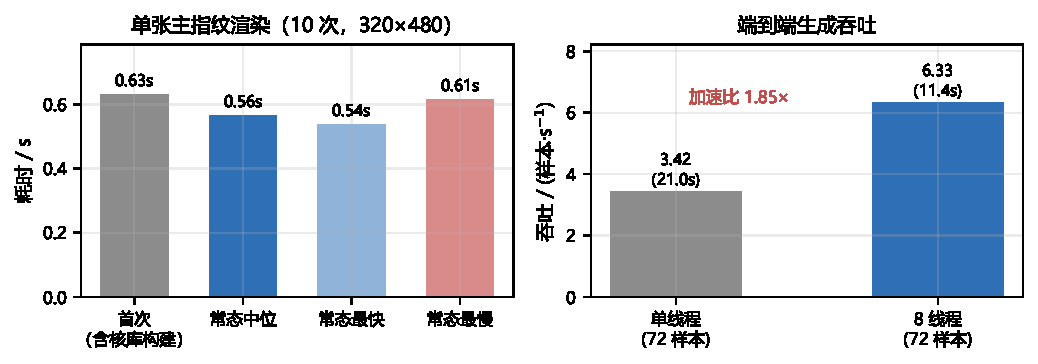
\includegraphics[width=0.98\textwidth]{figures/fig_perf.pdf}
\caption{生成性能。（a）单张主指纹渲染耗时；（b）端到端吞吐（72 样本，
每主指纹派生 4 样本）。}
\label{fig:perf}
\end{figure}

值得讨论的是并行加速比：8 线程相对单线程仅 $1.85\times$，远低于线性加速。
原因有二：其一，OpenCV 的滤波与重映射运算内部已做多线程，外层再并行会造成
线程超额订阅；其二，Python 层的调度、序列化与磁盘写入仍需解释器串行执行。

\subsection{质量与细节点}

72 个样本的质量分均值 $68.7$、中位 $71.6$、标准差 $11.0$，范围 $31.5$--$83.4$
（\figref{fig:quality}）。按等级统计，1--5 级分别为 7、44、14、6、1 个样本，
即多数样本落在 L2（较好），少量强退化样本落入 L4/L5，符合``随机退化链''的
设计预期。细节点数量均值 $80.6$、中位 $85$，范围 $0$--$117$。

\begin{figure}[H]
\centering
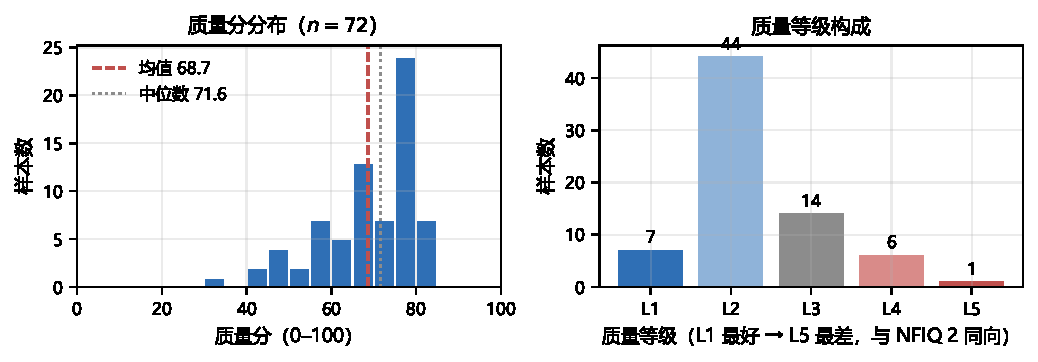
\includegraphics[width=0.98\textwidth]{figures/fig_quality.pdf}
\caption{质量评估结果。（a）质量分分布；（b）质量等级构成（L1 最好，与 NFIQ 2 同向）。}
\label{fig:quality}
\end{figure}

五类指纹的分布为：左箕 $24$、右箕 $24$、螺型 $12$、弓型 $6$、双箕 $6$，
与默认类别比例一致。数据集总体积 $8.87\unit{MB}$，平均每样本 $126\unit{KB}$
（含图像、掩模、方向场、细节点与质量图）。

\subsection{脊线几何真实性}
\label{sec:ridge}

合成指纹最容易被一眼识破的地方是脊线密度。真实 500\,dpi 指纹的脊线周期
（一脊一谷）约为 $8$--$12\px$。本文对 24 个未增强样本的 786 条扫描线做了
两种独立估计（\tabref{tab:ridge}、\figref{fig:ridge}）：自相关法给出中位
$11.0\px$（四分位 $9$--$16$），过零点计数法给出中位 $14.3\px$
（四分位 $10.1$--$19.5$），脊线占空比为 $0.50$。

\begin{table}[H]
\centering
\caption{脊线几何测量结果（24 个样本、786 条扫描线）}
\label{tab:ridge}
\small
\begin{tabular}{lccc}
\toprule
估计方法 & 中位周期 / px & 四分位区间 / px & 落入 8--12\,px 比例 \\
\midrule
自相关 & 11.0 & 9.0--16.0 & 54.5\% \\
过零点计数 & 14.3 & 10.1--19.5 & 38.2\% \\
\midrule
参考（真实 500\,dpi） & 8--12 & --- & --- \\
\bottomrule
\end{tabular}
\end{table}

两种估计整体一致，但过零点法系统性偏大：低对比度区域的脊线断裂会减少过零点
计数，从而把周期估大。综合来看，本系统生成的脊线周期与真实指纹同量级，
但\textbf{偏向区间上界}（略粗）。这与频率图的配置有关——默认允许
$5$--$15\px$ 的局部变化，其长周期端超出了真正常见的范围。若需要更贴近真实，
可在界面上把``最宽脊宽''下调至 $12\px$ 左右。

\begin{figure}[H]
\centering
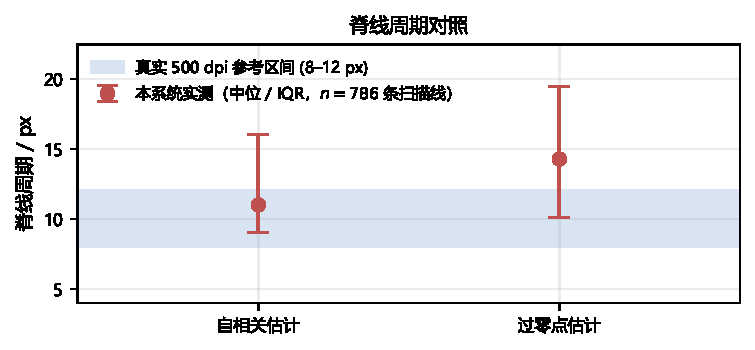
\includegraphics[width=0.72\textwidth]{figures/fig_ridge.pdf}
\caption{脊线周期与真实 500\,dpi 参考区间对照。点为中位值，误差棒为四分位区间。}
\label{fig:ridge}
\end{figure}

\subsection{可复现性验证}
\label{sec:repro}

以``同名数据集、同种子、不同输出目录''独立运行两次，比对
\texttt{checksums/sha256sums.txt}：504 个文件的 SHA-256 全部一致（差异 $0$）。
需要强调实验设计上的一个陷阱：由于数据集名称参与 dataset 级种子派生，
用\textbf{不同名称}重跑会得到完全不同的数据——这并非可复现性失效，而是设计使然。
最初的实验脚本正是踩了这个坑，导致误报；修正实验设计后结论才成立。

\subsection{实验中发现的缺陷及其修复}
\label{sec:defect}

首次正式实验中，72 个样本里有 4 个（$5.6\%$）出现``质量分 $0$、细节点 $0$、
掩模全黑、图像全白''。逐层排查后定位到\S 4.5 所述的掩模变换：掩模被纳入了
\textbf{全部} TTA 算子链，而亮度类算子会把归一化后的前景（$1.0$）压到阈值以下
（如 $\delta=-0.6$ 时变为 $0.4$，乘 $255$ 后低于 $127$），使掩模被整块清空；
随后背景还原逻辑把整幅图刷成纯 $255$。

修复方式是按算子类别过滤：只有几何与遮挡算子参与掩模变换，光度、噪声、压缩
与传感器算子跳过。修复后同一实验的空白样本比例由 $5.6\%$ 降至 $0$，质量分
标准差由 $19.0$ 收敛到 $11.0$。该问题已固化为回归测试：对二值掩模施加
亮度、对比度、Gamma 与噪声算子，断言掩模逐像素不变。

% =====================================================================
\section{讨论}

\subsection{与 SFinGe 的异同}

本文在方法学上沿用了 SFinGe 的``轮廓—奇异点—方向场—频率图—Gabor''主线，
但在工程取向上有四点不同：其一，依赖从数十个缩减到 4 个，便于在受限环境中
部署；其二，把捺印的``形变 / 传感器 / 退化''拆成三段独立开关，使研究者能按
实验需要控制变量；其三，将可复现性机制化（种子树 + 校验和），而非依赖使用者
自行记录；其四，提供图形界面与命令行双入口，前者降低使用门槛，后者便于脚本化
与批处理。

\subsection{局限性}

\begin{enumerate}
    \item \textbf{缺少识别级评测。}本文的评测集中在生成侧（性能、质量分布、
          脊线几何、可复现性），尚未在统一协议下比较``合成数据训练的识别模型''
          与``真实数据训练的模型''的性能差距。这需要配套的指纹匹配器与公开测试
          协议，超出本期工作量。
    \item \textbf{脊线周期略偏粗。}如 \S\ref{sec:ridge} 所述，默认参数下脊线
          周期偏向 $8$--$12\px$ 区间的上界，且允许的局部变化范围偏宽。
    \item \textbf{并行加速比有限。}8 线程仅 $1.85\times$，与 OpenCV 内部并行
          造成的线程超额订阅有关，后续可考虑限制 OpenCV 线程数再与外层并行组合。
    \item \textbf{质量分未标定。}自研评分器与 NFIQ 2 同向但未做等级映射标定，
          跨数据集比较时应谨慎。
\end{enumerate}

\subsection{后续工作}

近期计划包括：接入开源指纹匹配器（如 minutiae-based 基准算法）建立识别级评测；
把脊线周期与占空比纳入持续集成，作为``真实感''的守护指标；引入按像素质量图
加权的 CFAR 级联筛选，提高低质量样本的可用性；以及在生成后端上预留接口，
以便与基于深度学习的生成方法做对照实验。

% =====================================================================
\section{结论}

本文围绕``如何低成本、合规、可复现地获得指纹数据''这一问题，设计并实现了桌面
平台 \name{}。它复刻了 SFinGe 的生成方法学，并以工程手段解决了轻量部署、
逐字节可复现与插件化扩展三个实际约束。72 样本的正式实验表明：单张主指纹渲染
中位耗时 $0.57\unit{s}$，8 线程端到端吞吐 $6.33$ 样本/秒；质量分均值 $68.7$、
细节点均值 $80.6$；脊线周期与占空比与真实 500\,dpi 指纹处于同一量级；
同配置同种子两次独立运行的 504 个文件校验和完全一致。实验期间还定位并修复了
一个会导致 $5.6\%$ 样本静默失效的掩模缺陷。

我们认为，这类``把研究原型做成可用工具''的工作，其价值不仅在于算法复刻本身，
更在于它把可复现性、可核查性与可维护性变成了默认属性——这正是合成数据能够被
他人放心用于论文与产品的前提。

% =====================================================================
\phantomsection
\addcontentsline{toc}{section}{参考文献}
\bibliography{refs}

% =====================================================================
\appendix
\section{复现命令}

\begin{lstlisting}[language=bash, float=htbp, caption={从零复现本文数据集}, label={lst:repro}]
# 1) 环境（4 个核心依赖 + 一个 Qt 绑定）
pip install -r requirements.txt

# 2) 自检：17 项，含"同种子两次渲染逐像素一致"
python -m synthfp selfcheck

# 3) 生成本文实验数据集（72 样本）
python -m synthfp generate \
    --set dataset.name=paper_demo \
    --set dataset.identities=6 \
    --set dataset.fingers_per_identity=2 \
    --set dataset.impressions_per_finger=2 \
    --set dataset.tta_per_impression=3 \
    --set runtime.workers=8 \
    --set runtime.seed=2026

# 4) 校验（重算 SHA-256 并比对清单）
python -m synthfp validate --dataset outputs/paper_demo --check-hash
\end{lstlisting}

\section{数据集体结构}

\begin{lstlisting}[language=bash, float=htbp, caption={输出目录结构}, label={lst:layout}]
outputs/paper_demo/
  README.md                  数据集说明（含合成声明与复现方法）
  dataset_manifest.jsonl     每行一个样本的完整记录（唯一元数据来源）
  plan.jsonl                 生成计划（可复现依据）
  config.resolved.yaml       实际生效的完整配置
  environment.json           环境快照 + 配置指纹
  stats.json                 统计报告
  splits/{train,val,test}.csv 按身份划分，杜绝身份泄漏
  checksums/sha256sums.txt   全量文件校验和
  images/000001/left_thumb/imp_01/000001_left_thumb_imp01_tta00.png
  mask/  orientation/  minutiae/  quality/  logs/
\end{lstlisting}

\section{种子派生伪代码}

\begin{lstlisting}[language=Python, float=htbp, caption={层级种子树（SHA-256 派生）}, label={lst:seed}]
def stable_seed(*parts: object) -> int:
    text = "|".join(str(p) for p in parts)
    digest = hashlib.sha256(text.encode("utf-8")).digest()
    return int.from_bytes(digest[:8], "big")

def derive(base_seed: int, *parts: object) -> int:
    return stable_seed(base_seed, *parts)

# dataset -> identity -> finger -> impression -> tta
ds   = derive(root_seed, "dataset", dataset_name)
idt  = derive(ds, "identity", identity_id)
fng  = derive(idt, "finger", finger)
imp  = derive(fng, "impression", impression_index)
tta  = derive(imp, "tta", tta_index)
\end{lstlisting}

\end{document}
